\chapter{算法实现和性能评估}
本章节主要评估了前一章节三种策略的性能优化效果,包括减少关键帧间隔,智能丢帧策略GreedyDrop,以及最后的整套方案,GVBR算法。在本文所有的仿真实验中,我们将帧率都设置为30帧每秒。

\section{最佳GOP}
\ref{sec:design_space}章节的初步实验验证表明减小关键帧间隔可以降低丢帧。但减少关键帧间隔实际上是个很棘手的选择,因为关键帧数目的增加可能会导致视频质量的降低。在本节中,我们尝试去具体评估由于减少关键帧间隔所带来的性能变化。

\textbf{视频质量和关键帧} 关键帧间隔的选择需要在视频质量和丢帧数之间达到一个动态均衡。为了指导关键帧间隔的选择,我们重复进行了多次实验,每次实验改变关键帧间隔大小,将未压缩的视频流压缩成H264格式,测量压缩后的视频画面质量。实验中使用x264编码器~\cite{x264}~\cite{lai2017furion}去编码原始视频,实验中需要进行编码的原始视频为同一视频片段。x264编码器工作在差分编码模式,两个关键帧之间相隔的帧越多越有可能引起累计误差,GoP的推荐值是小于250帧。虽然最大限制值为250帧,但具体的关键帧间隔取值依然很复杂。我们使用的视频数据集包含各种不同类型的视频,超清视频,高清视频,游戏和4k视频~\cite{video}。关键帧间隔大小和归一化SSIM的关系展示在图~\ref{fig:ssim_gop}中,SSIM的单位值为一次实验中最大的SSIM值。我们从众多视频集中挑选出四组视频,代表整体的实验结果。从图中可以看出,当关键帧间隔大于0.5秒后,由于编码器压缩量化导致的视频质量损失很微小,SSIM的数值基本保持不变,在最大SSIM的(97\%-100\%)范围内。结合前面对关键帧间隔和丢帧数的关系的测量,选择小的关键帧间隔会减少丢帧数。总结上面的实验,我们给出了关键帧的建议选择范围$[0.5,2]$秒。

\begin{figure}[htb]% use float package if you want it here
  \centering
  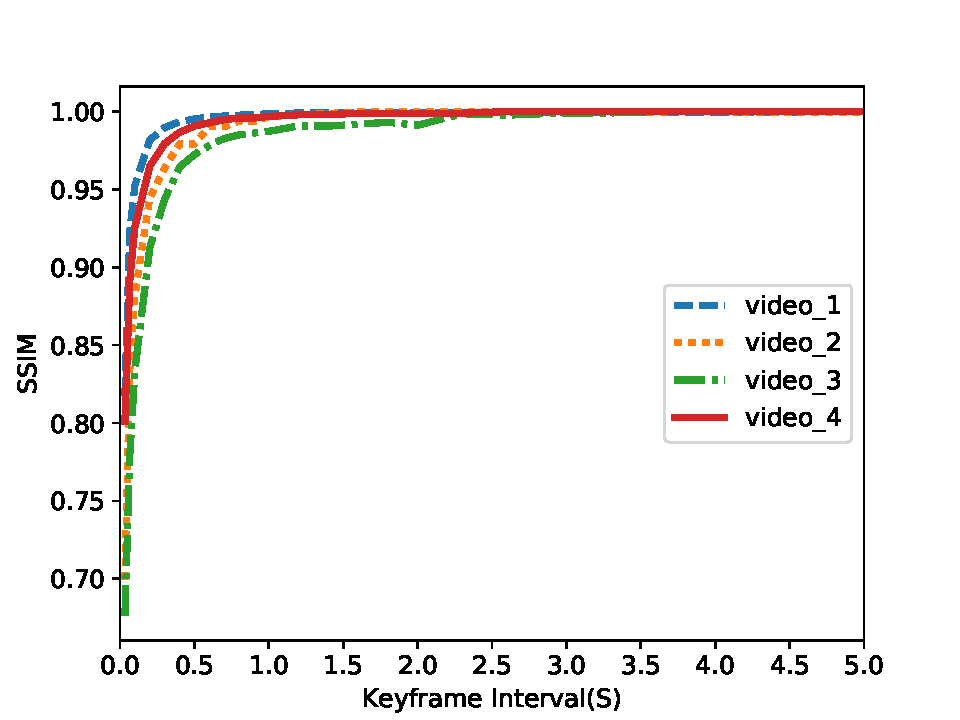
\includegraphics[width=0.7\textwidth]{ssim_gop}
  \caption{不同关键帧间隔时视频编码后的SSIM}
  \label{fig:ssim_gop}
\end{figure}

\section{智能丢帧策略}
\subsection{智能丢帧策略的实现}
为了衡量丢帧算法的性能优化效果,我们选择了两个算法作为对比,离线最优算法Oracle和默认算法OBS。Oracle,通过暴力搜索加剪枝可以达到离线最优,但其时间复杂度在指数级别。我们从带宽数据集中任意选择其中一段,时长为30秒附近。利用上一小节的结论,关键帧间隔的选择范围为$[0.5,2]$秒,我们将关键帧间隔设置为1秒。为了研究算法优化丢帧的效果,在三组实验中我们将码率都固定在2850kbps,小于初始带宽值,但远大于衰落之后的带宽值。合理的码率选择使得这段数据既包含长时间的带宽抖动,也包括瞬时的带宽抖动。视频的帧率依然选择为30帧每秒。

GreedyDrop算法的具体实现见流程图~\ref{fig:GreedyDrop}。每当一个新的视频帧产生时,会启用图中的机制去处理视频帧。首先,判断和P帧相关的丢帧优先级是否被置为$True$,如果被置为$True$,则丢弃视频帧队列中时间较为久远的视频帧,直到碰到I帧时才会停止丢帧,将队列时间跨度在原有值的基础上减去丢帧时长。另外,如果视频帧队列中存在关键I帧的话,则将丢帧优先级置为$False$。其次,下面的步骤则是在满足带宽约束的条件下尽可能多的发送视频帧,将队列时间跨度在原有值的基础上减去已发送的时长。最后,判断现在的时间跨度是否大于阈值$T1$,如果大于P帧的阈值,则丢弃视频队列中所有不满足及时性约束的帧,同时将队列的时间跨度减去丢弃的时长,将丢帧优先级置为$True$。一个视频帧的完整处理机制就是这样,完成对于视频帧的处理后便等待着一个新的视频帧产生,以触发上述机制。
\begin{figure}[htb]
    \centering
    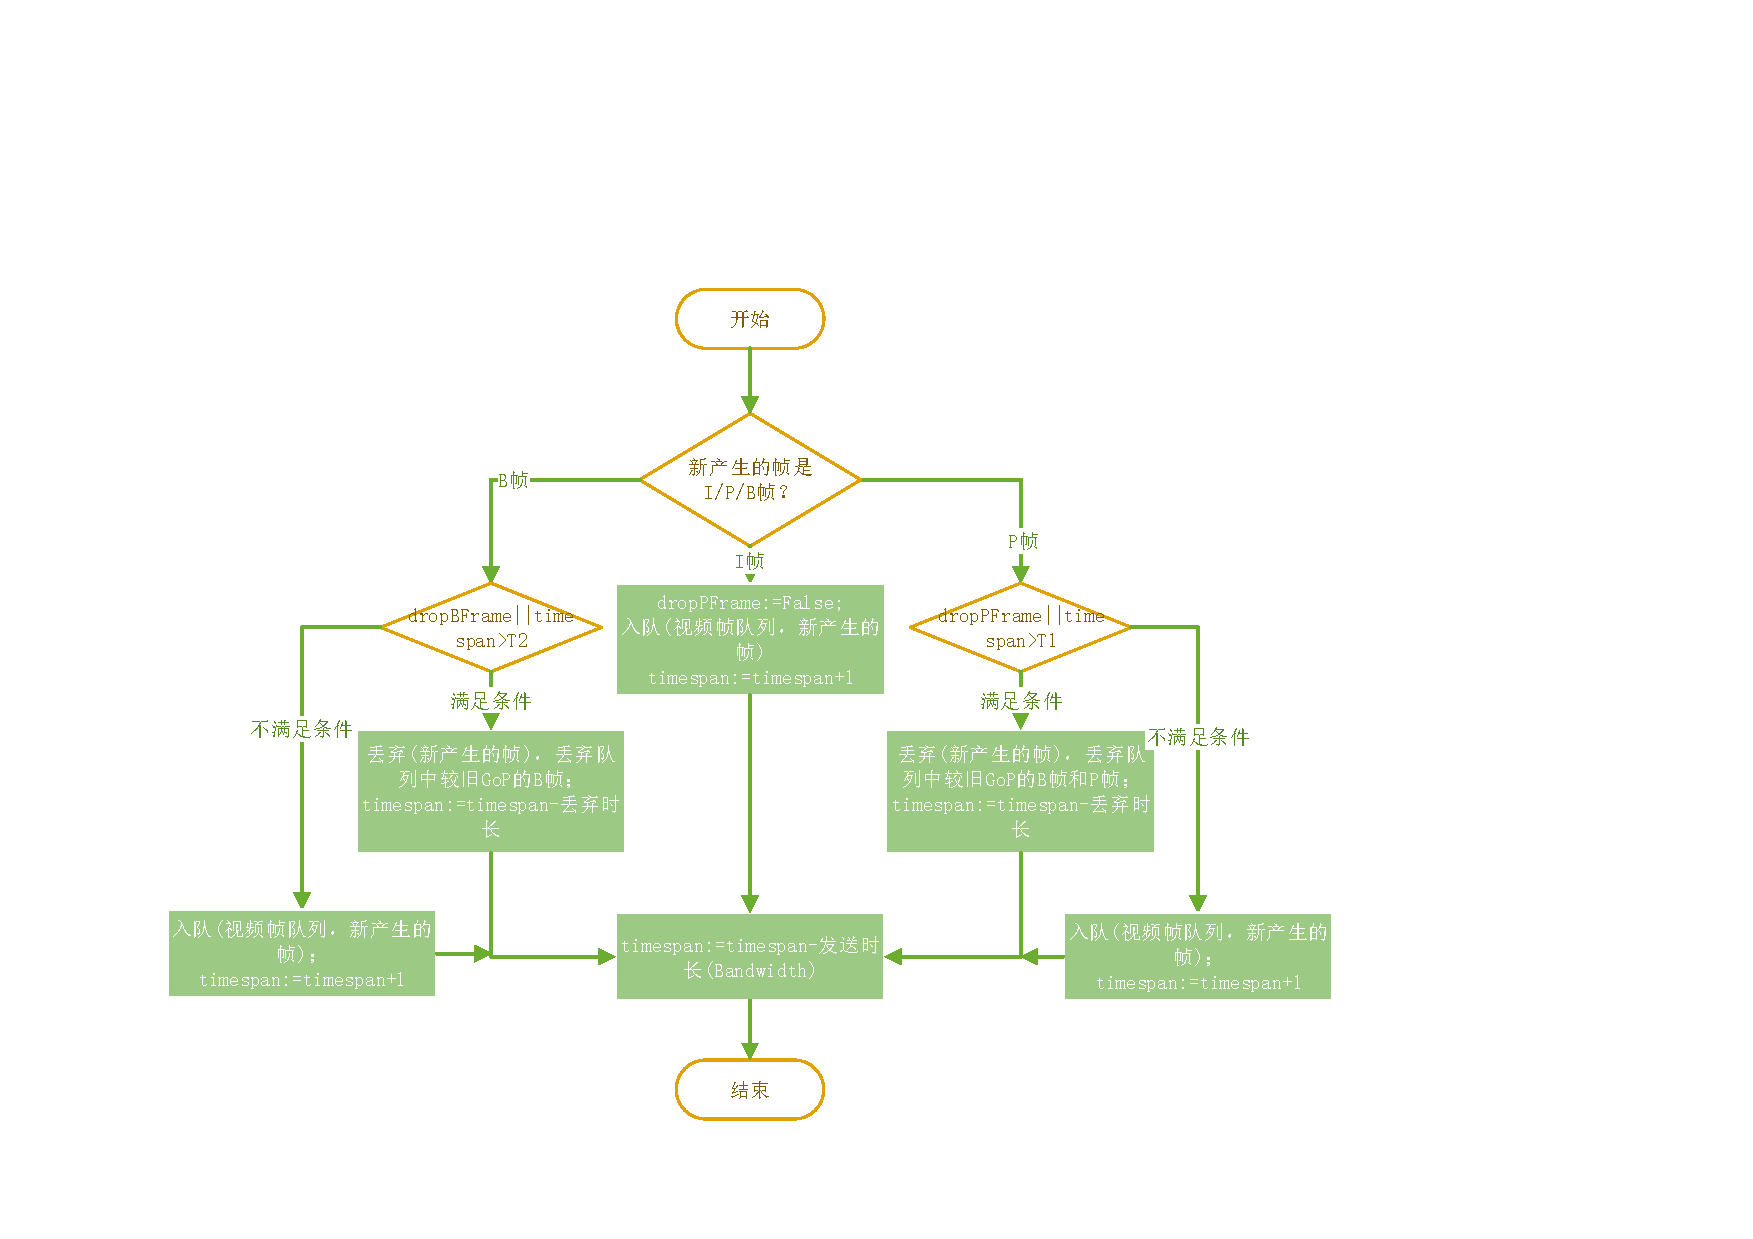
\includegraphics[width=0.5\linewidth]{GreedyDrop}
    \caption{GreedyDrop算法的实现流程图}
    \label{fig:GreedyDrop}
\end{figure}

离线最优丢帧算法Oracle的核心代码部分如图~\ref{fig:Oralce}所示。对于每个时隙来说,可能的丢帧策略数和视频帧队列中GoP的组数有着相关关系。对于视频帧队列中的帧排列,丢帧首先需要满足可解码性的要求,即丢帧之后队列中剩余的视频帧都必须可以正常解码。所以一个合理的丢帧策略是,对于视频帧队列中的每一个GoP,丢弃每个GoP组结尾连续的视频帧。Oracle算法的核心代码部分用递归的想法来实现,对于每个GoP,列出所有可能的丢帧组合,并继续往下递归直到循环的GoP组数等于队列包含的GoP组数。具体例子如下所示,例如,对于一个含有k个帧的GoP来说,合理的丢帧策略总共有k种,即,丢弃0个帧,丢弃最后一个帧,丢弃最后两个帧...丢弃最后k-1个帧和丢弃所有的帧。对于每一个GoP来说,从k种情况中选择一种,继续循环下一个GoP的情况,所以对于一个有N个GoP的视频帧队列来说,丢帧情况的组合数为指数次复杂度。由于Oracle算法的复杂度过高,因此在仿真实验时,我们只取了30秒时隙的数据集用来仿真。
\begin{figure}[htb]
    \centering
    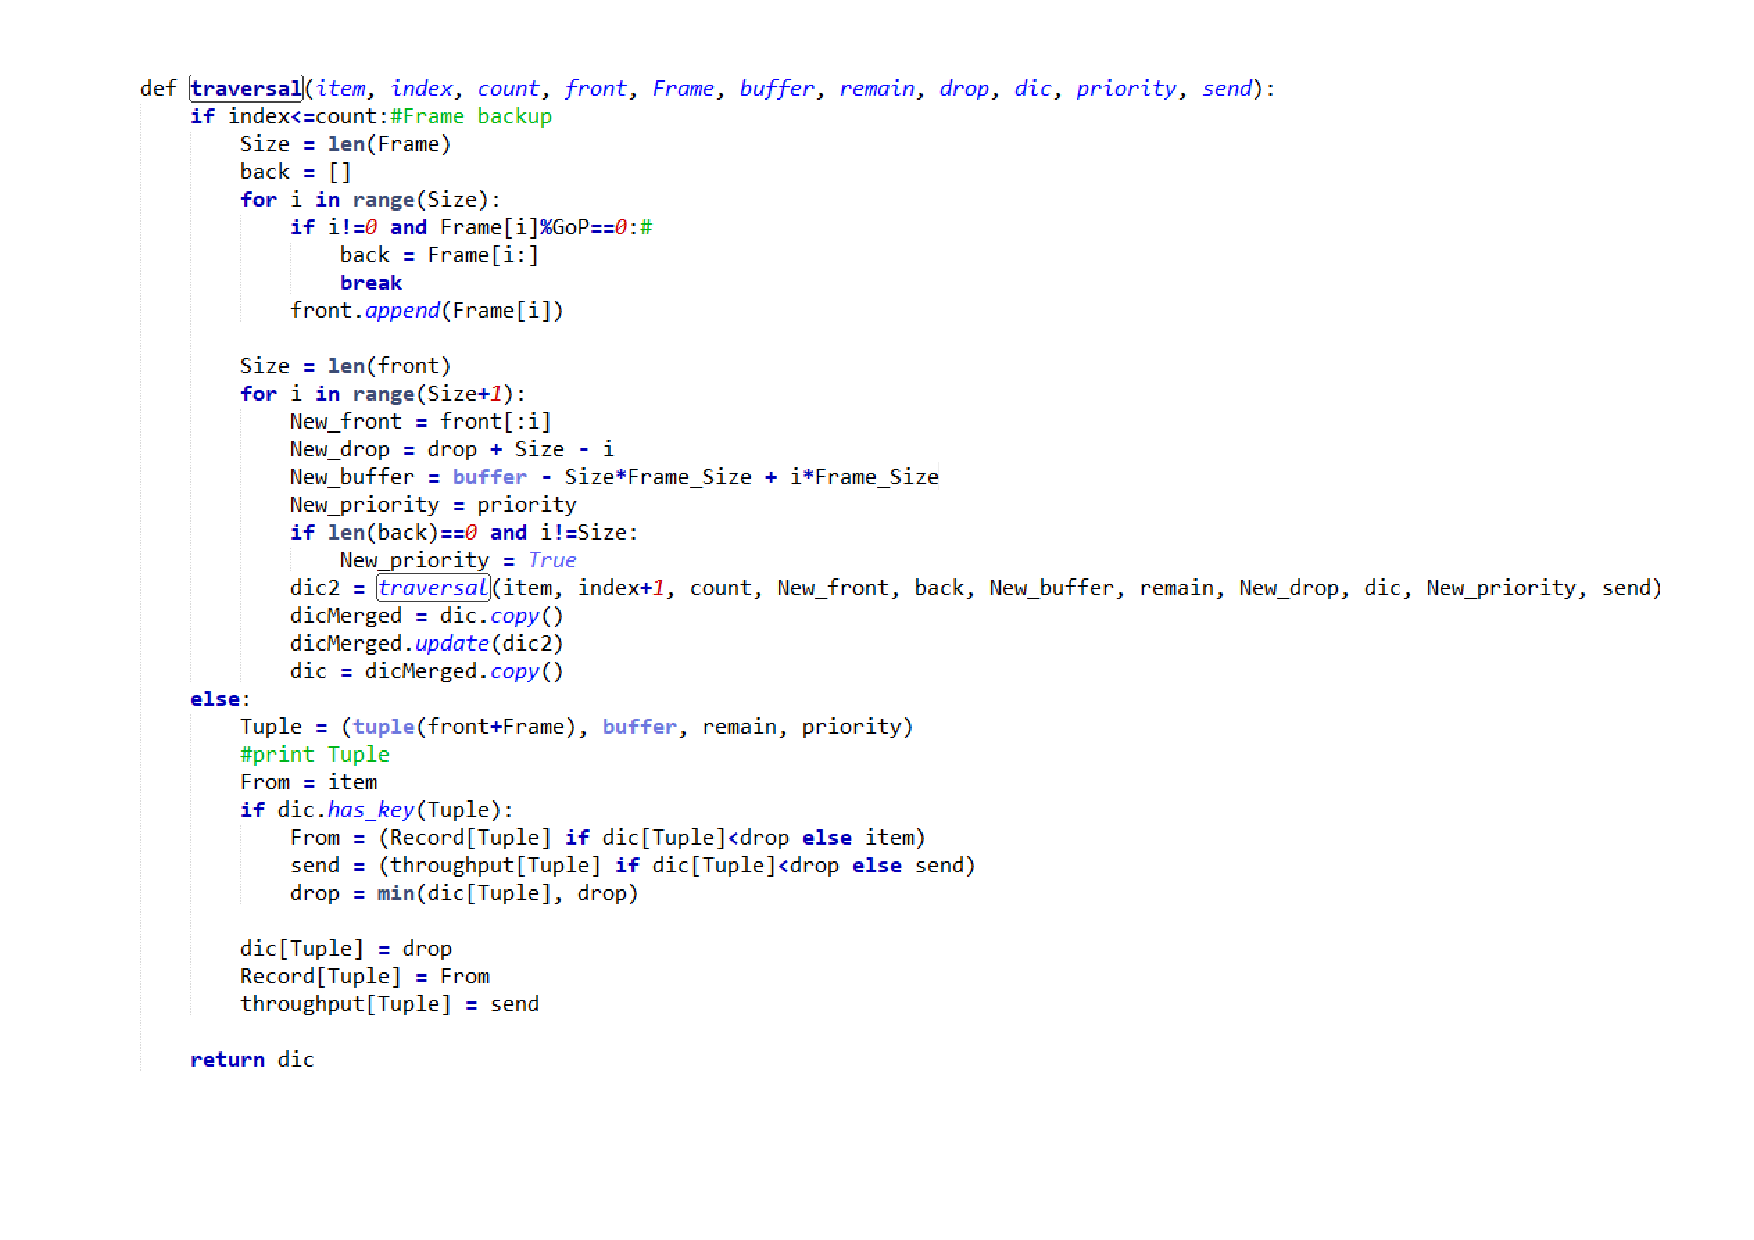
\includegraphics[width=1\linewidth]{Oracle}
    \caption{离线最优算法Oracle的具体实现}
    \label{fig:Oralce}
\end{figure}

\subsection{丢帧策略的效果评估}
\begin{figure}[tb]
  \centering%
  \begin{subfigure}{0.49\textwidth}
    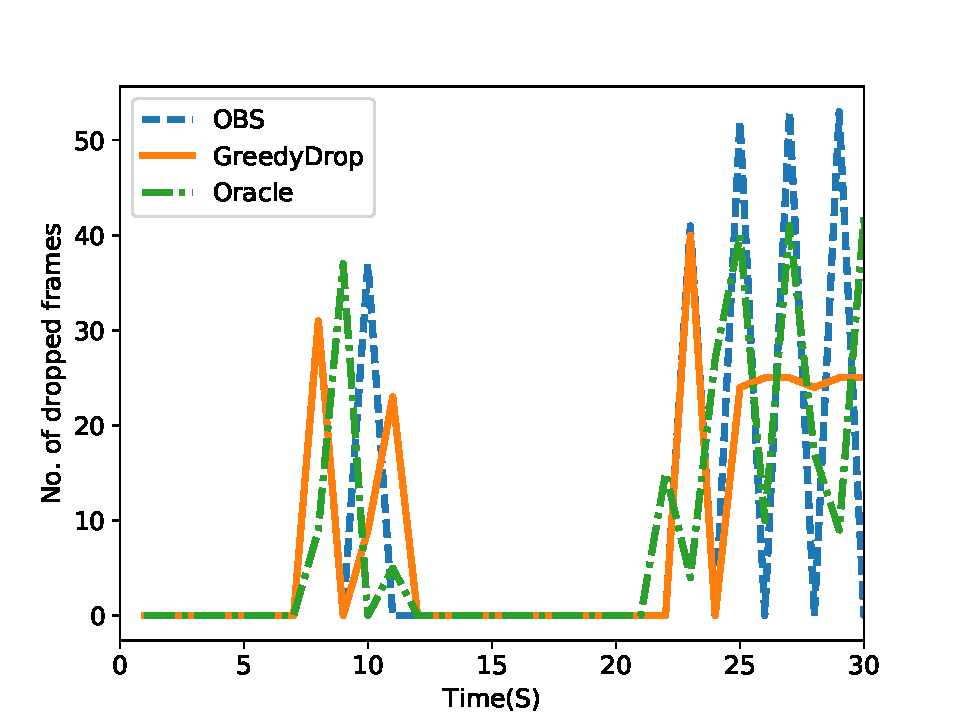
\includegraphics[width=\textwidth]{drop-buffer}
    \caption{实时丢帧数}
    \label{fig:drop-buffer}
  \end{subfigure}%
  \hfill
  \begin{subfigure}{0.49\textwidth}
    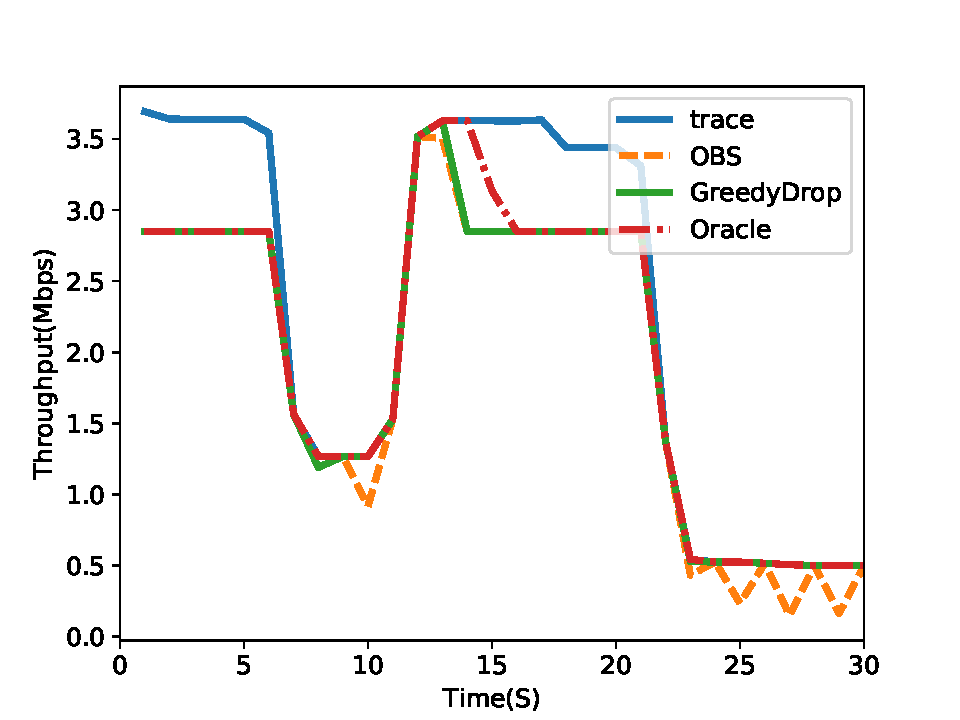
\includegraphics[width=\textwidth]{drop-bandwidth}
    \caption{实时的吞吐量}
    \label{fig:drop-bandwidth}
  \end{subfigure}
  \vspace{0.1in}
  \caption{不同丢帧策略性能比较}
  \label{fig:drop_comparison}
\end{figure}

在该数据集下,三种算法丢帧的减少程度在表~\ref{tab_drop}中给出。本文中,我们定义了一个新的指标来衡量算法的性能,上传失败时长。上传失败时长定义为丢帧数对应的播放时长,计算方式为丢帧数除以每秒的帧数。

\begin{table}[tb]
\centering
\caption{与默认OBS算法相比丢帧的减少程度}
\label{tab_drop}
    \begin{tabularx}{\linewidth}{cccX}
    \toprule[1.5pt]
    \textbf{算法} &\textbf{丢帧数} &\textbf{上传失败时长(秒)} & \textbf{与默认OBS算法相比丢帧对应的百分比}    \\ \midrule[1pt]
    Oracle    &265  &8.83  &$80\%$           \\
    GreedyDrop  &274 &9.13  &$85.6\%$              \\
    OBS默认算法     &320  &10.67  &无 \\
    \bottomrule[1.5pt]
\end{tabularx}
\end{table}

三种算法中,默认的OBS丢帧算法丢帧数最多,上传失败时长最长,高达10秒,GreedyDrop智能丢帧算法减少了15\%的上传失败,将上传失败时长降低到9.13秒,改善丢帧的效果较为明显。而且GreedyDrop在线算法和离线最优Oracle算法之间的差距较小,约等于5\%左右,离线最优算法的上传失败时长仅为8.8秒。实时丢帧数和真实吞吐量的时序图展示在图~\ref{fig:drop_comparison}中。丢帧主要发生的时间段位于7到12秒和20到30秒期间。7到12秒时三种算法的表现基本相同,实时带宽紧跟控制数据一起变化;因为Oracle算法知道网络恢复的具体时间,相对于其他算法,会在视频队列中保存更多的有效帧,当网络状况恢复后,10到15秒期间时Oracle算法会将队列中的视频帧以burst的形式发送出去,相比于其他两个算法,避免了一部分丢帧。20到30秒期间,网络经历着长时间的带宽抖动,OBS算法的丢帧数呈现周期性的振荡变化,方差很大,而GreedyDrop算法基本每个时刻的丢帧都很稳定。因为GreedyDrop算法只丢弃视频队列中属于旧的GoP的帧,而OBS算法每次丢帧将队列中的帧全部丢弃,因为丢帧行为会呈现一定的周期性。对于GreedyDrop算法,每个GoP开头的帧被发送出去,剩余的帧都被丢弃,规律性的行为使得丢帧数和吞吐量都保持恒定。Oracle算法和OBS算法的性能类似,每个时刻的丢帧数有一定的波动,但是方差变化比较小。同时考虑时间复杂度和算法性能,GreedyDrop是个不错的选择。

\section{自适应码率算法}
\subsection{自适应码率算法实现}
我们选取了几个在视频点播方面性能很好的动态码率算法,作为对比算法,来和GVBR算法做比较。为了控制变量,保持对比算法的一致性,和GVBR算法一样,对比算法中我们依然用调和平均值来作为对带宽的预估。
\begin{itemize}
  \item OBS-VBR:简单直接的码率自适应算法,和OBS默认算法基本一致,使用OBS默认的丢帧策略,唯一的不同点在于动态码率,每个时刻都选择比估计带宽低的最高可用码率。
  \item MPC:用队列状态信息(帧数和帧的大小,以及帧的类型)和预测带宽值去计算接下来几个时隙的最优码率选择,但只应用第一个时隙的码率选择,对于之后的时隙重复上述过程。
  \item Robust-MPC:使用和MPC类似的方法,唯一的不同点,在于用过去几个时隙的最大预测误差去矫正未来几个时隙的带宽估计。
\end{itemize}
除了OBS-VBR算法之外,上述的几个对比算法均用GreedyDrop作为丢帧策略。Robust-MPC是视频点播领域最先进的码率自适应算法,MPC算法和Robust-MPC算法均是使用模型预测控制理论去选择未来时隙的码率。模型预测控制理论,简称MPC,主要的思想是预测未来几个时隙的带宽和系统状态,计算几个时隙的最优选择,但在应用时只用第一个时隙的选择,这个理论可以直接应用到直播场景中去,因此我们选择将Robust-MPC和MPC作为我们的直播动态码率对比算法。

GVBR算法具体实现的流程图如图~\ref{fig:GVBR}所示。每当新的视频帧产生时,触发图中的机制去处理视频帧。本文中码率选择的粒度为一个GoP,所以如果新产生的视频帧是关键帧I帧的话,那么必须进行的过程是为该GoP选择一个合适的码率。码率的选择需要根据历史带宽信息以及视频帧剩余的数据量大小来确定。记录过去5个GoP期间的真实带宽$[C_{j-5},C_{j-1}]$,求其调和平均值$C_j$,作为该时隙的预估带宽。$C_j$的具体计算公式如下:
\begin{eqnarray}
% \nonumber % Remove numbering (before each equation)
  &&   C_j = 1/(\sum_{k=j-5}^{k=j-1} 1/C_k)
\end{eqnarray}
。另外,考虑到视频帧队列里剩余的数据量$Rest$,循环扫描整个比特率数组,找到一个最大的码率$Rate$使得满足以下约束条件:
\begin{eqnarray}
% \nonumber % Remove numbering (before each equation)
  &&   0.9*Rate+Rest<C_j
\end{eqnarray}
。当选定当前GoP的码率值后,剩下的操作和视频帧为非关键帧相同。首先,在满足带宽约束的条件下,尽可能多的发送队列里的视频帧;之后,判断目前的视频帧队列是否满足及时性要求,即队列里是否存在$T1$时间之前产生的视频帧,弱存在,丢弃所有$T1$之间的视频帧。同时为了保证发送的视频帧都具有可解码性,丢弃和前一步丢帧有约束关系的视频帧。上述过程完整的叙述了视频帧产生后的处理机制,处理完成后,GVBR算法等待下一个视频帧的产生。
\begin{figure}[htb]
    \centering
    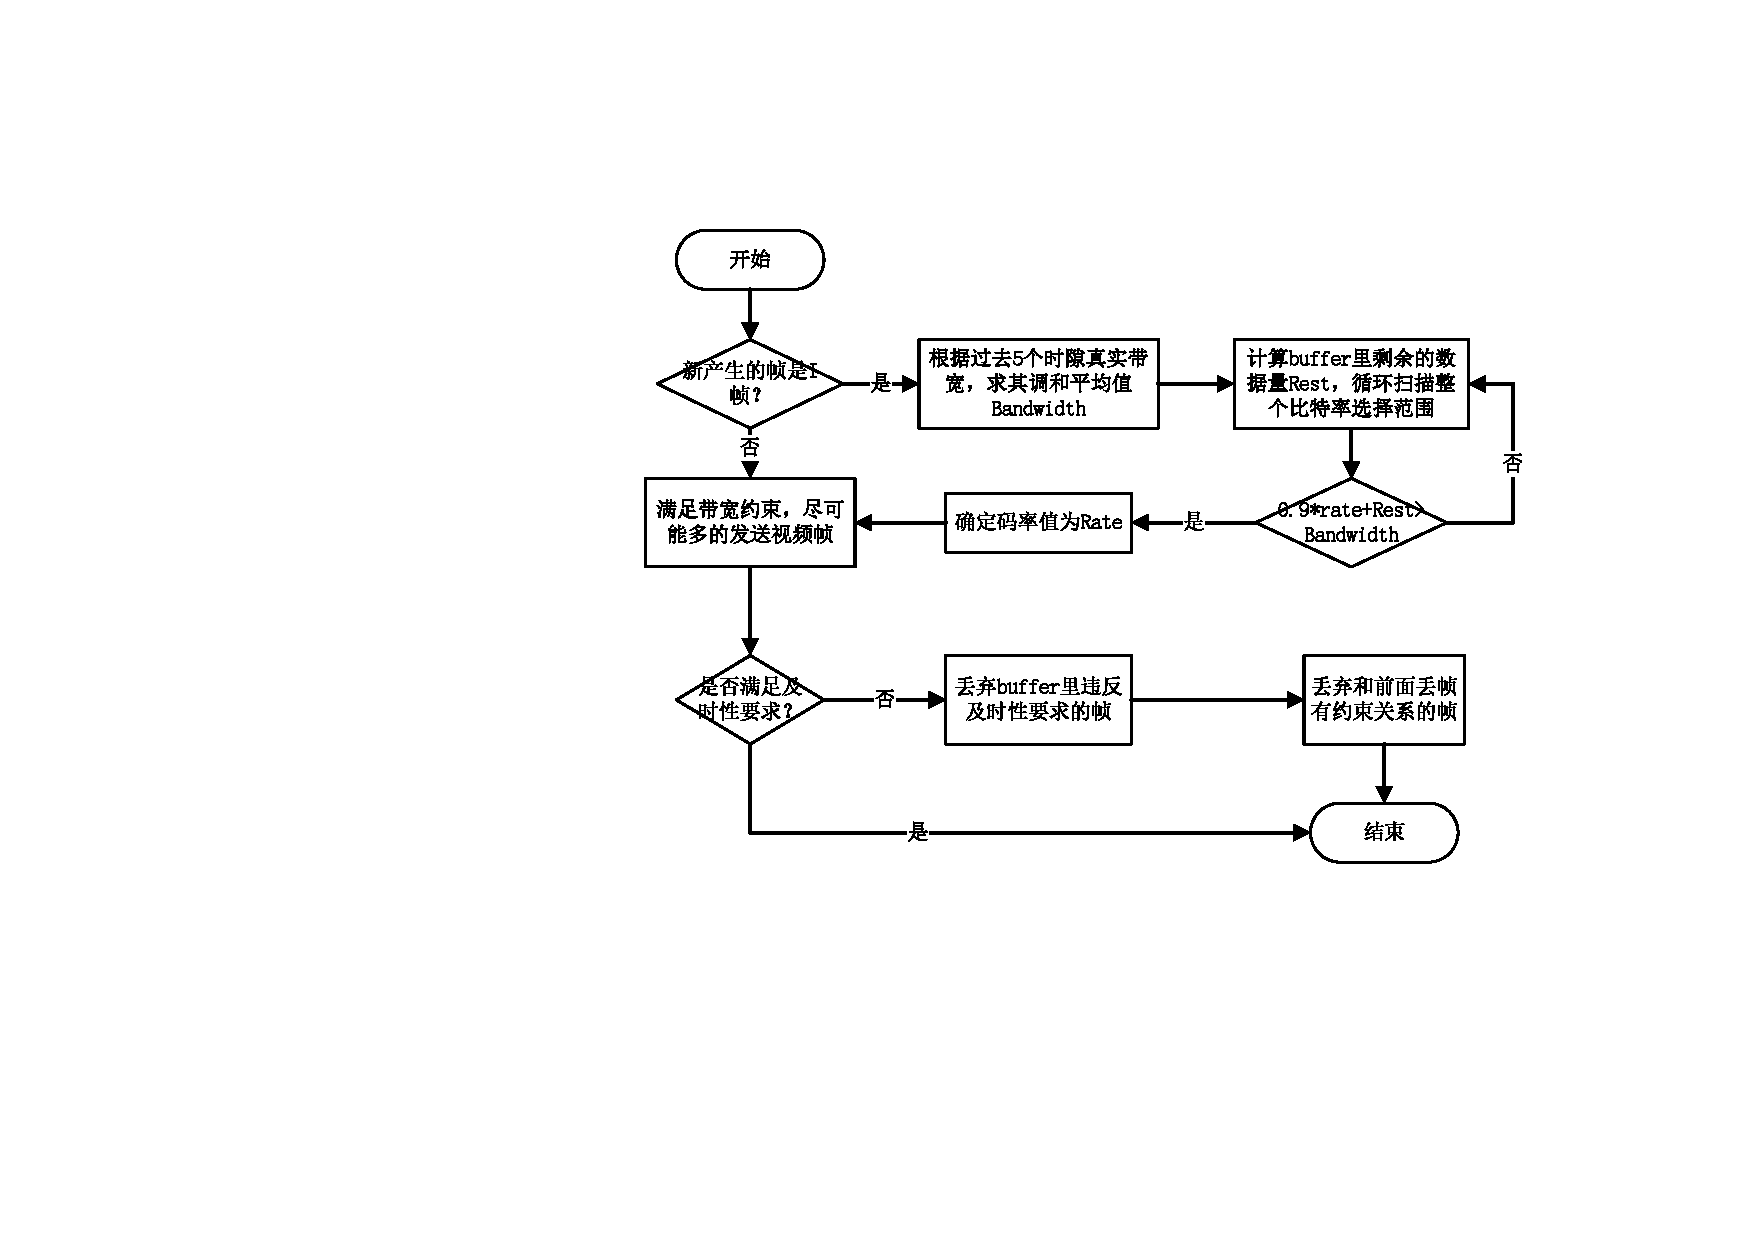
\includegraphics[width=0.9\linewidth]{GVBR}
    \caption{GVBR算法的实现流程图}
    \label{fig:GVBR}
\end{figure}

Robust-MPC算法相比于MPC算法增加了带宽纠正的部分,用过去几个时隙的预测误差去纠正当前时隙MPC算法对于带宽的预估,具体的代码实现如图~\ref{fig:bandwidth_correction}。$Esm_history$为记录的过去$\tau$个时隙的真实带宽值,$Error$为对于预测带宽的纠正参数。$Error$等于过去$\tau$个时隙中最大的预测误差比,如代码所示。由于增加了对于带宽预估的纠正,Robust-MPC相对于MPC算法来说,性能得到明显的改善。
\begin{figure}[htb]
    \centering
    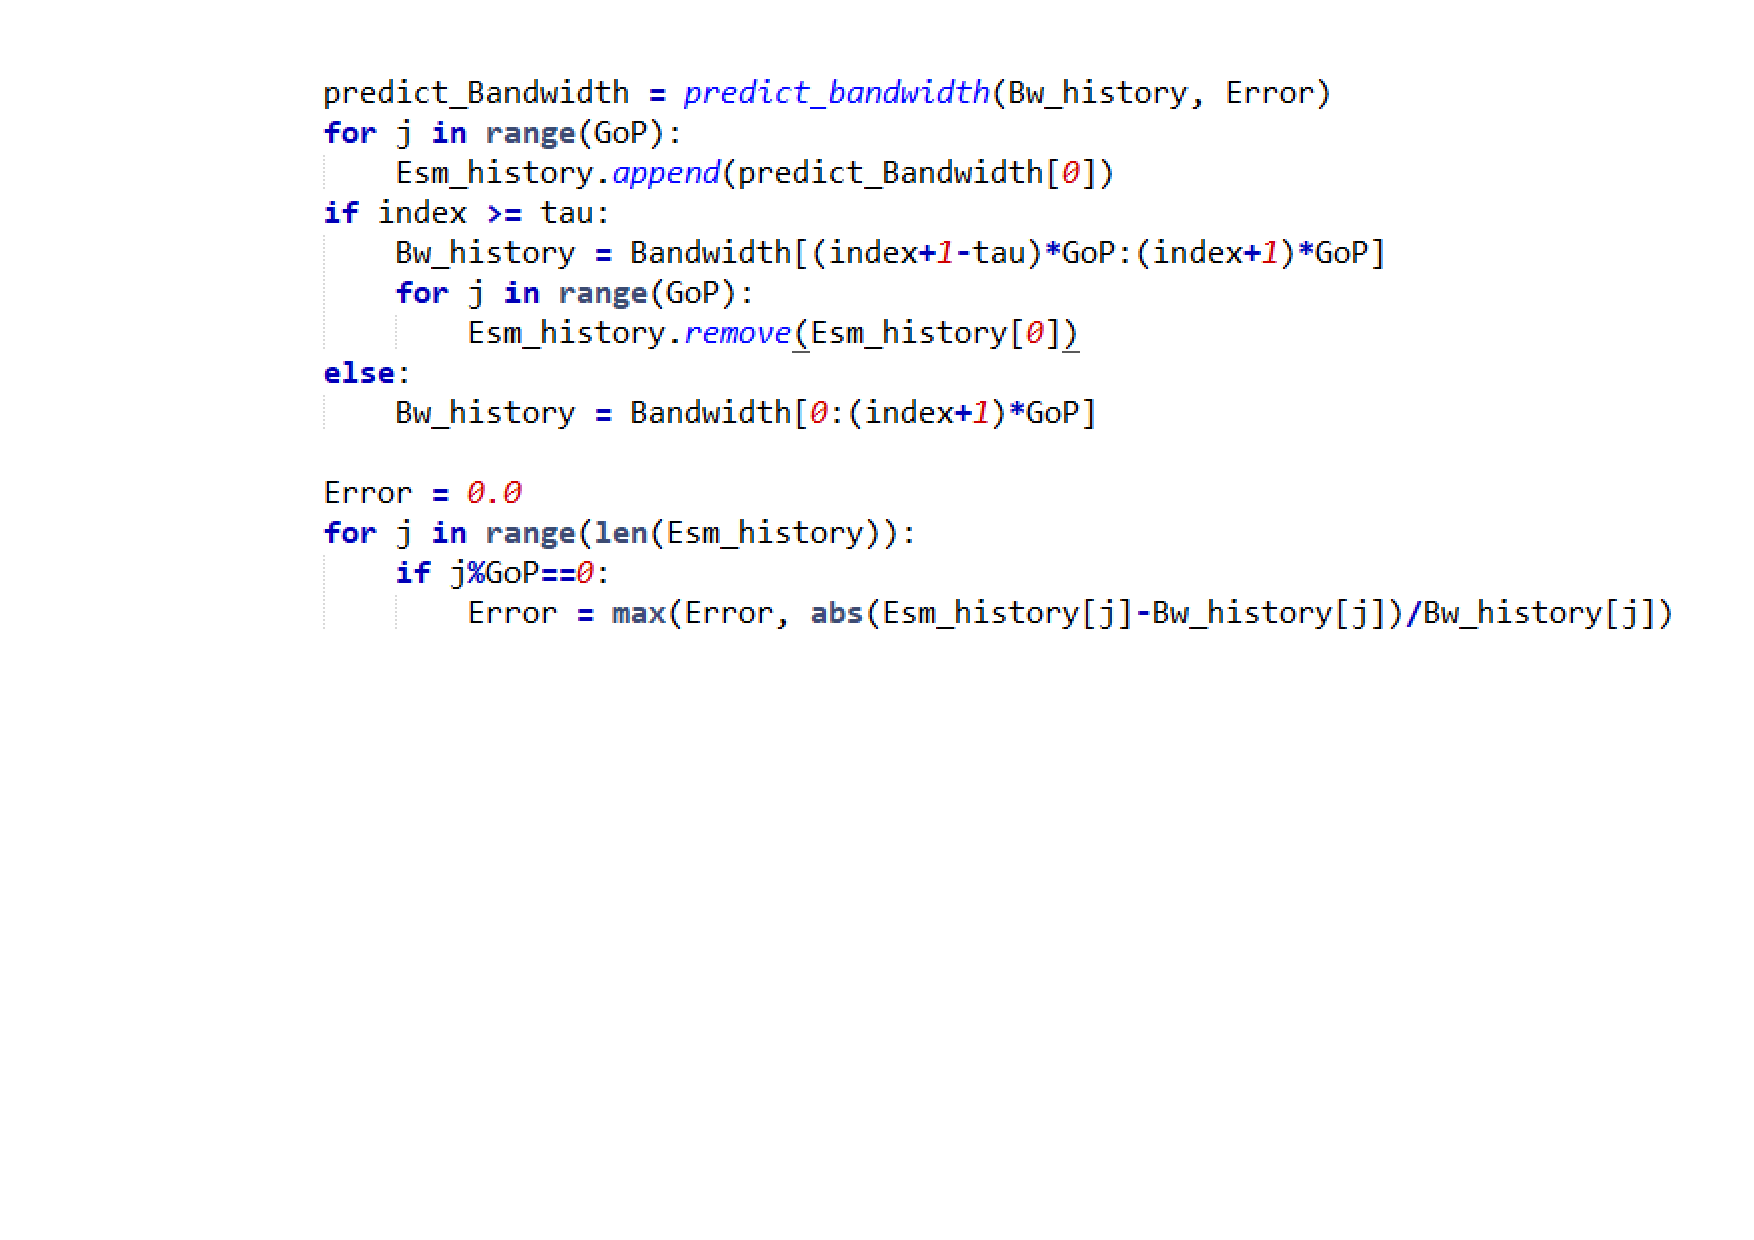
\includegraphics[width=0.9\linewidth]{BandwidthCorrection}
    \caption{Robust-MPC算法中带宽纠正的代码实现}
    \label{fig:bandwidth_correction}
\end{figure}

图~\ref{fig:MPC}是MPC算法和Robust-MPC算法的公共部分,给出了在未来$\tau$个时隙如何选择最优的码率组合。对于未来的$\tau$个时隙,假设每个时隙可选择的码率有$M$个,所有的码率组合数达到$M^\tau$。循环扫描所有的码率组合,对于任一码率组合,模拟未来$\tau$个时隙的具体过程,记录总的丢帧数,计算每一码率组合可以获得的总效益。找出最大效益对应的码率组合,并在接下来的一个GoP应用该码率选择,循环上述过程。MPC和Robust-MPC的具体实现就是这样。
\begin{figure}[htb]
    \centering
    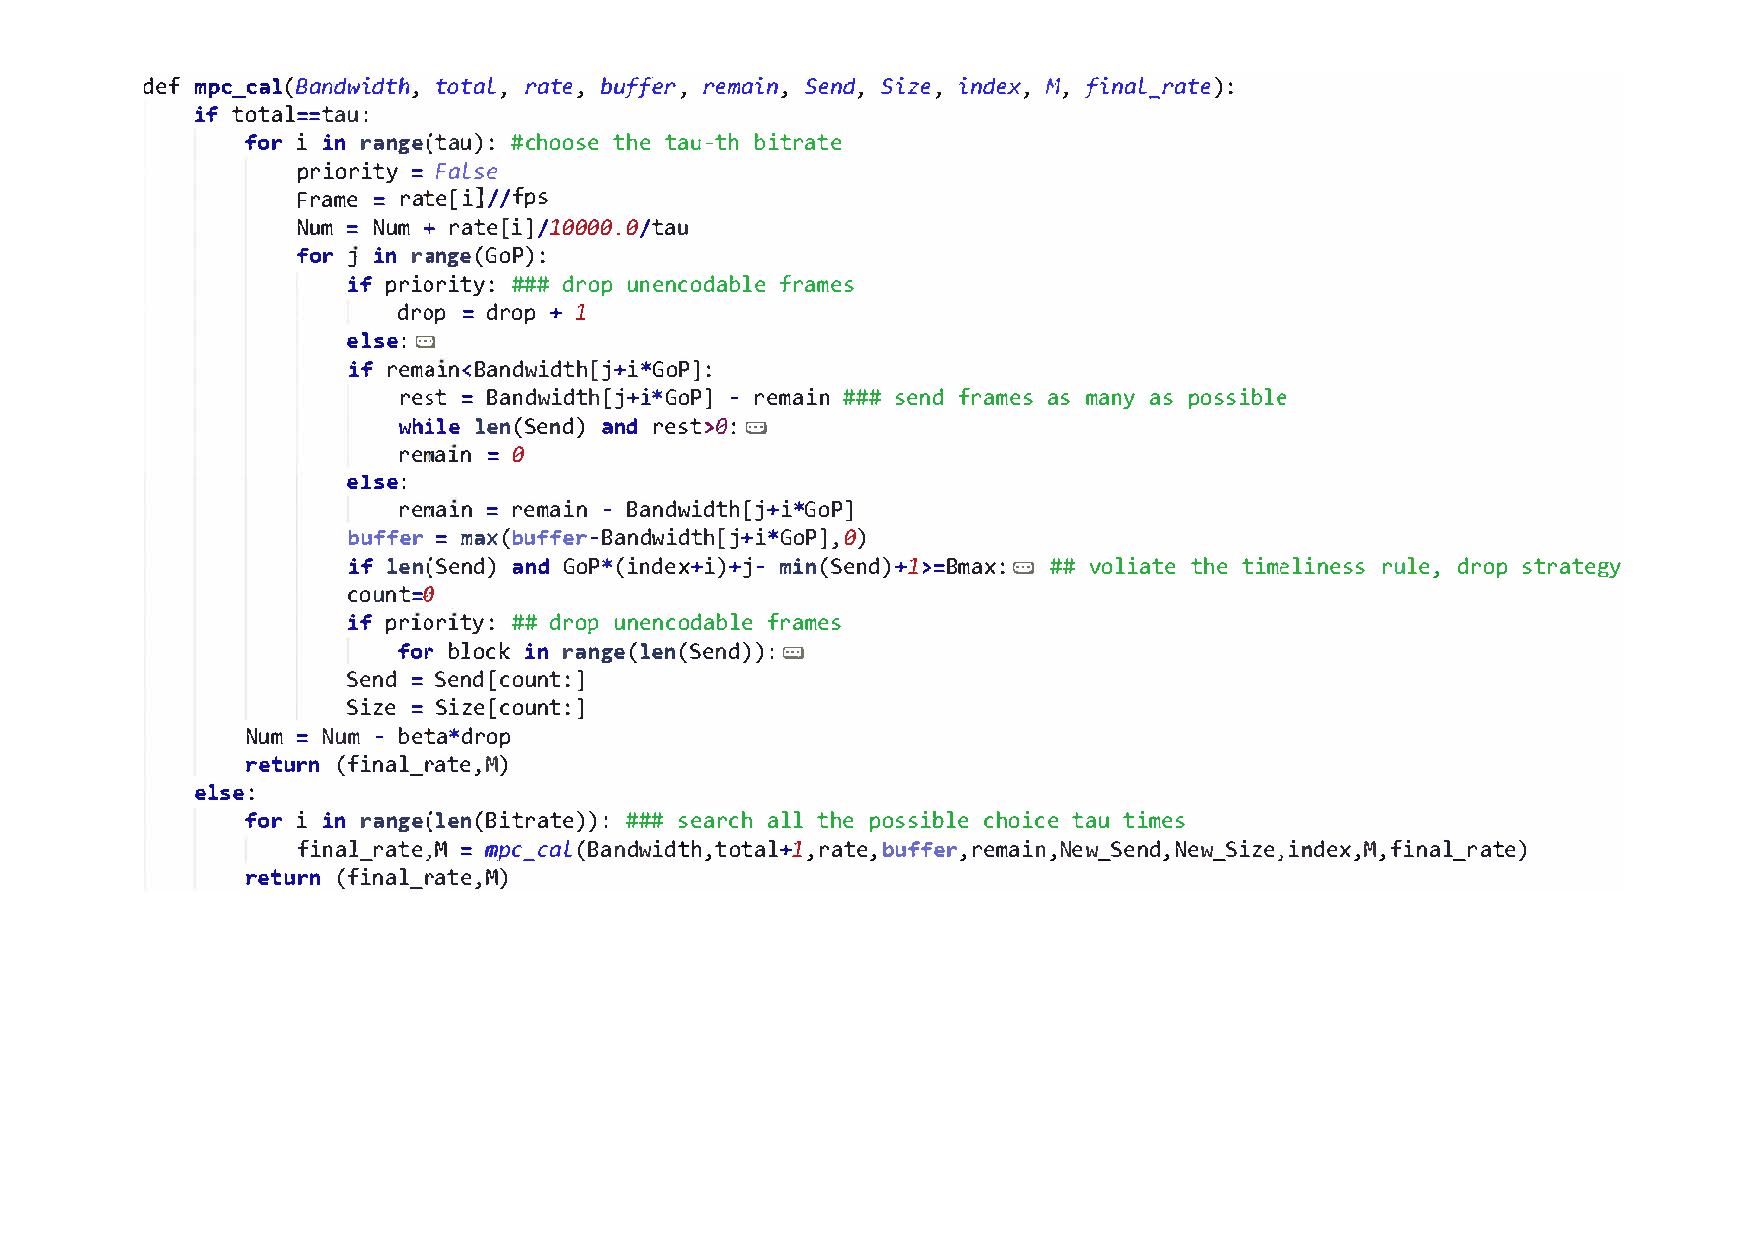
\includegraphics[width=\linewidth]{MPC_algorithm}
    \caption{MPC和Robust-MPC未来几个时隙最优码率选择的代码实现}
    \label{fig:MPC}
\end{figure}

\subsection{码率自适应算法效果评估}
\begin{figure}[tb]
  \centering%
  \begin{subfigure}{0.5\textwidth}
    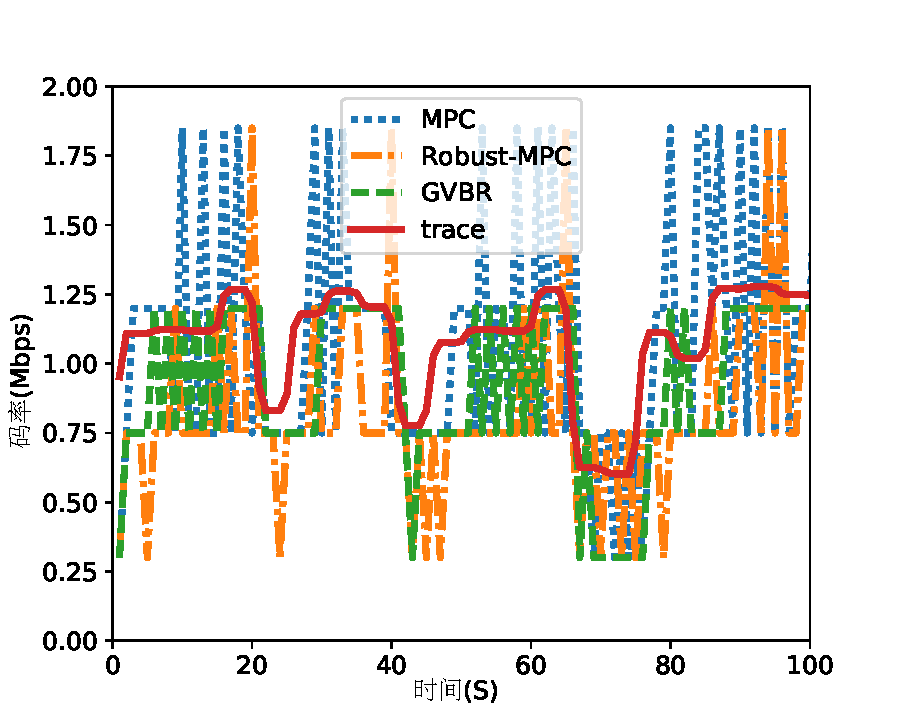
\includegraphics[width=\textwidth]{specific_fcc}
    \caption{FCC数据集的实时吞吐量}
    \label{fig:fcc}
  \end{subfigure}%
  \hfill
  \begin{subfigure}{0.5\textwidth}
    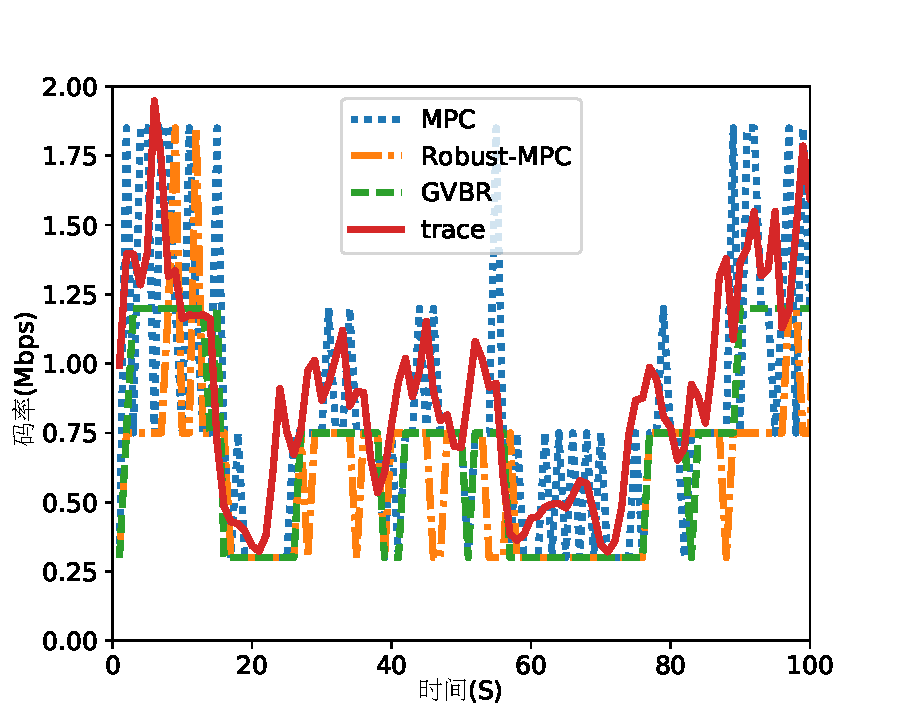
\includegraphics[width=\textwidth]{specific_hsdpa}
    \caption{HSDPA数据集的实时吞吐量}
    \label{fig:hsdpa}
  \end{subfigure}
  \vspace{0.1in}
  \caption{不同码率自适应算法吞吐量比较}
  \label{fig:specific}
\end{figure}

详细的对比算法结果展示在图~\ref{fig:specific}中。图~\ref{fig:fcc}和图~\ref{fig:hsdpa}分别展示了FCC数据集和HSDPA数据集下三种算法的性能。在这两幅图中,实线代表着真实世界的带宽数据记录。相比于Robust-MPC,MPC缺少对预测误差的矫正,容易更激进的选择更高的码率,反映到图中,MPC每个时刻的码率总是高于Robust-MPC的码率。除此之外,两个MPC算法的码率总是在真实带宽附近波动。两种数据集下,MPC和Robust-MPC的码率切换都比GVBR更频繁。这是因为GVBR的策略是选择比带宽低的最高码率,当带宽波动较小时,GVBR很有发生变化。但是MPC的策略是选择一个使用户体验质量最高的码率,当带宽稍微波动一点,MPC会更加倾向于选择一个更高或码率,增大优化目标中的第一项,码率相关的效益。而Robust-MPC虽然增加了对于预测误差的矫正,但依然是求几个时隙的最优选择,和MPC的行为较为类似。

\begin{figure}[tb]% use float package if you want it here
  \centering
  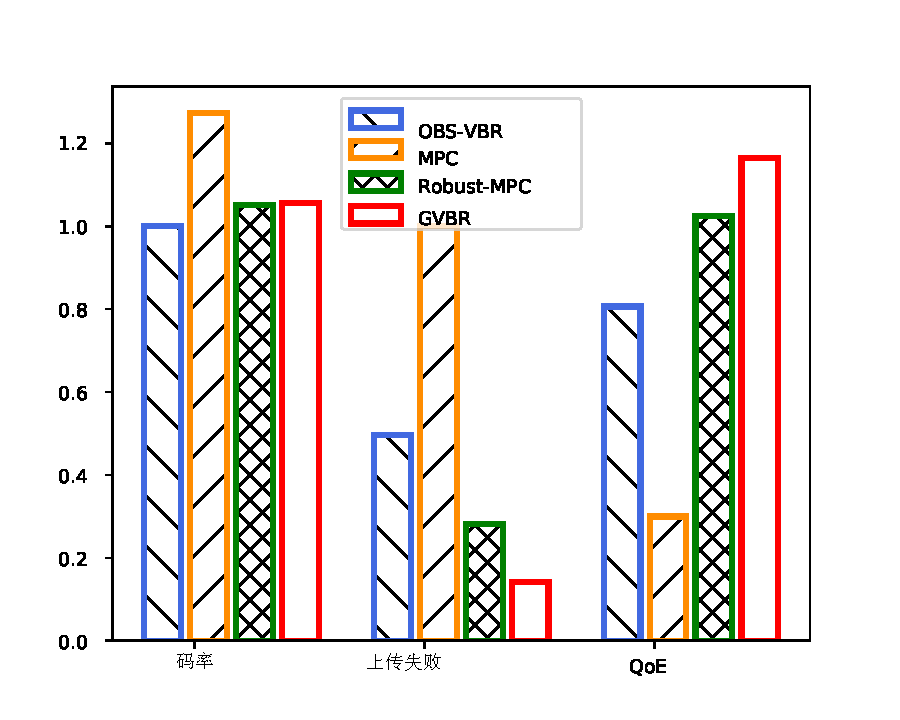
\includegraphics[width=0.7\textwidth]{massive_qoe}
  \caption{归一化平均码率,上传失败时长和用户体验质量}
  \label{fig:massive_qoe}
\end{figure}

大规模的仿真实验的具体结果展示在图~\ref{fig:massive_qoe}中,我们结合两个数据集去综合评估GVBR算法的性能,两个数据集分别是FCC数据集和HSDPA数据集。图中展示的三项指标,平均码率,上传失败时长以及用户体验质量都是归一化之后的平均指标。综合对比四种算法,MPC算法拥有最高的码率效益,这是因为MPC的带宽估计算法很激进,会更倾向于选择较高的码率。其他三种算法有着基本相同的平均码率,其中GVBR和Robust-MPC两种算法的平均码率稍微高一点,高于OBS-VBR算法。虽然MPC达到了最高的码率水平,但也带来了最高的丢帧数,对应的平均上传失败的时间也最长。OBS-VBR算法使用的丢帧算法是默认的OBS丢帧策略,所以在剩余三种算法中上传失败的时长最高。Robust-MPC算法相对于MPC算法来说增加了对于预测误差的纠正,将上传失败时间减少到可以忍受的时长。因为考虑了队列中排队等待发送的视频帧的数据量,GVBR将平均上传失败的时长减少到很少的时间,相对于Robust-MPC减少了50\%左右。平均码率略微高于多个对比算法,而且平均上传失败时长很短,GVBR的用户体验质量在所有算法中达到了最高水平。剩余三种算法的用户体验质量排序分别是Robust-MPC,OBS-VBR和MPC。

\begin{figure}[tb]
  \centering%
  \begin{subfigure}{0.48\textwidth}
    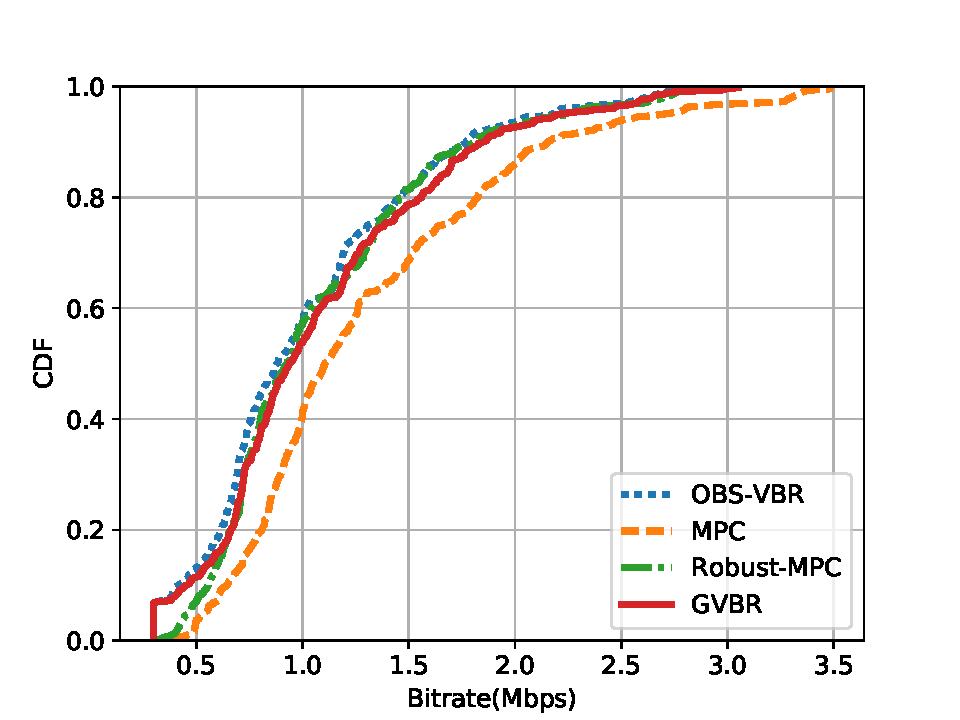
\includegraphics[width=\textwidth]{massive-bitrate-cdf}
    \caption{平均码率累计分布图}
    \label{fig:bitrate_cdf}
  \end{subfigure}%
  \hfill
  \begin{subfigure}{0.48\textwidth}
    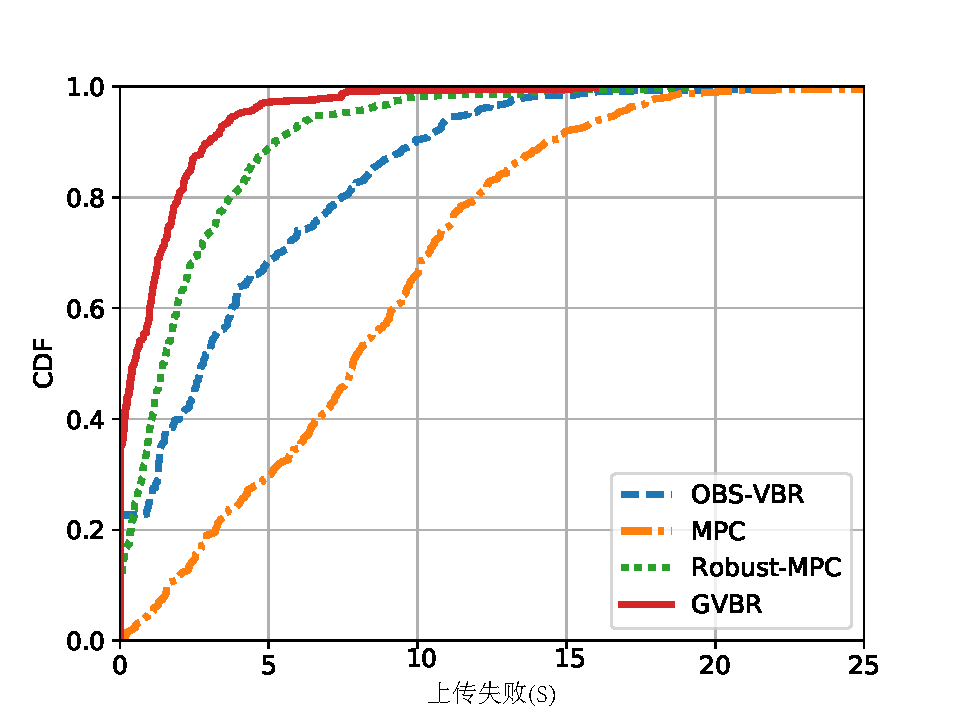
\includegraphics[width=\textwidth]{massive-drop-cdf}
    \caption{上传失败时长累计分布图}
    \label{fig:drop_cdf}
  \end{subfigure}
  \vfill
  \vspace{0.2in}
  \begin{subfigure}{0.48\textwidth}
    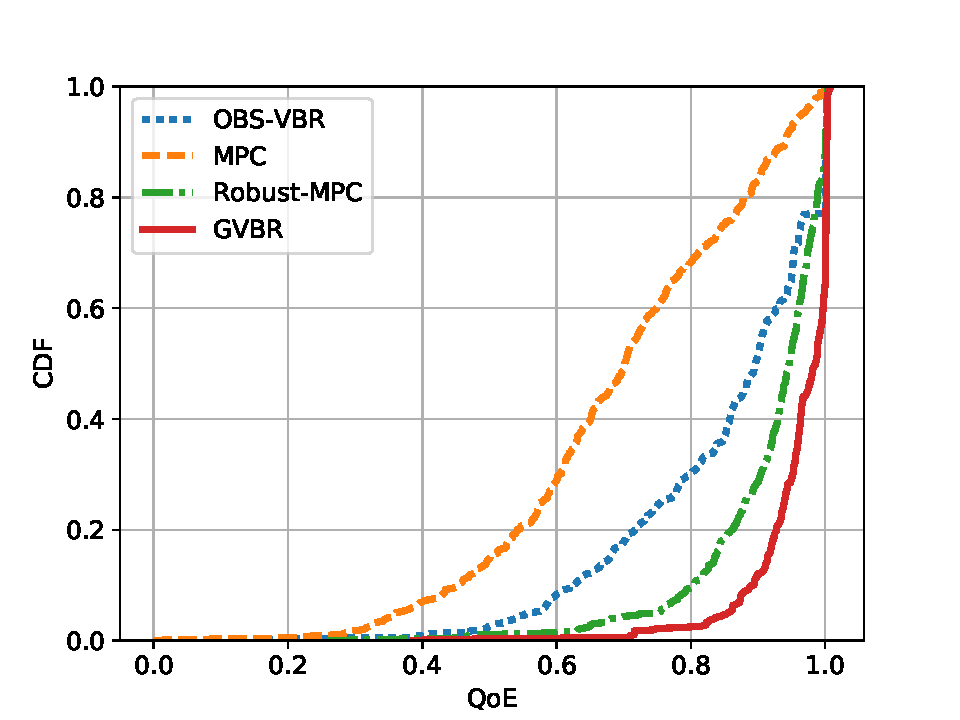
\includegraphics[width=\textwidth]{massive-qoe-cdf}
    \caption{归一化用户体验质量累计分布图}
    \label{fig:qoe_cdf}
  \end{subfigure}
  \vspace{0.1in}
  \caption{大规模实验结果图}
  \label{fig:massive_cdf}
\end{figure}

平均码率,平均上传失败时长和平均用户体验质量的累计分布图展示在图~\ref{fig:massive_cdf}中。在图~\ref{fig:bitrate_cdf}中,GVBR算法位于Robust-MPC和OBS算法的右边,码率值稍微高于这两者。
MPC位于其余三种算法的右边,码率值远远高于其他三种算法,和图~\ref{fig:massive_qoe}的结论一致。从图~\ref{fig:drop_cdf}中可以看出,对于GVBR算法,98\%的实验其上传失败时间都低于5秒,有大约40\%的的实验中未出现过上传失败。
而其余三种算法低于5秒上传失败时间的百分比分别是,Robust-MPC有90\%的实验上传失败时长低于5秒,OBS-VBR有70\%的实验,MPC只有30\%的实验。
图~\ref{fig:qoe_cdf}显示,GVBR算法只有2\%的实验中用户体验质量不是很好,其余的98\%的情况下归一化用户体验质量大约在$[0.8,1]$之间。剩余三种算法的归一化用户体验质量大于80\%的比例分别是,MPC为30\%,OBS-VBR为70\%,Robust-MPC为90\%。
总而言之,我们的GVBR算法在上传失败时长和用户体验质量两个指标上远远优于其他几个算法。

\begin{table}[tb]
\centering
\caption{码率自适应算法效果对比}
\label{tab:vbr}
\begin{tabularx}{\linewidth}{cccX}
\toprule[1.5pt]
\textbf{算法} &\textbf{平均码率(Mbps)} &\textbf{平均上传失败时长(秒)} & \textbf{平均用户体验质量}    \\ \midrule[1pt]
OBS    &1.0788  &26.1438  &-39107.835           \\
OBS-VBR  &1.0256 &3.9763  &-5862.833         \\
MPC     &1.3060  &8.0017  &-11877.126 \\
Robust-MPC &1.0781 &2.2553 &-3281.921 \\
GVBR &1.0821 &1.1414 &-1605.033 \\
\bottomrule[1.5pt]
\end{tabularx}
\end{table}

由于固定码率的OBS默认算法和其他四种自适应码率算法的性能差别过大,上述性能比较图中并未出现与默认OBS算法的对比结果。我们将默认OBS算法和几种动态码率算法的对比结果整理在表~\ref{tab:vbr}中。相比于最原始的固定码率的OBS算法,我们提出的GVBR算法减少了95.6\%的丢帧数。
默认的OBS算法其平均上传失败时长为26秒左右,而我们的GVBR算法只有1秒的平均失败时长。所有的算法除了MPC算法之外,GVBR算法在其中拥有最高的平均码率,略微高于其他三种算法。总的来说,我们的GVBR算法在达到更高的码率的基础上,显著减少了上传失败现象的发生。另外,
表~\ref{tab:vbr}中可以得到的重要结论是,在主播端引入自适应码率算法之后可以大幅度减少上传失败现象的发生。

\section{本章小结}
本章对于提出的优化方案进行了系统的性能评估,主要包括不同层面的方案,GoP层面的减少关键帧间隔以及码率自适应算法,GoP内部的智能丢帧策略。

首先,本章针对关键帧间隔大小对视频质量的影响进行了评估,发现了当关键帧间隔减少到一定值之后,视频质量呈现急剧下降,严重损害用户的观看体验。
为了避免这种现象,关键帧间隔在选取时应严格遵循最小取值的约束,减少丢帧现象发生的同时保证视频质量。

其次,对于棘手的丢帧策略选择,我们对比了离线最优算法和GreedyDrop算法的优劣。相比于默认的OBS丢帧策略,GreedyDrop和离线最优算法的性能明显优于前面两者。
但是离线最优算法的时间复杂度为指数级,对于移动设备的计算性能要求太高,而且离线最优算法需要已知全程的带宽状况,这在实际中是不可行的。综合时间复杂度和对于减少丢帧的性能改善,GreedyDrop算法是较优的选择。

最后,对于我们最后提出的一整套的解决方案GVBR,进行了充分的性能评估。不仅与视频点播领域较为先进的码率自适应算法MPC对比,而且和最原始的默认OBS算法进行了对比。
实验结果显示,除了在平均码率的指标上略逊色于MPC算法,在平均上传失败时长和用户体验质量方面远远优于其他几种算法。